\documentclass{article}

\usepackage[margin=0.5in,bottom=1in,footnotesep=1in]{geometry}

\usepackage{amsmath}


\usepackage{multicol}
\setlength{\columnsep}{1cm}
\usepackage[]{algorithm2e}

\usepackage{lipsum}% for dummy text
\usepackage[varg]{txfonts}
\usepackage{graphicx}
\usepackage{subcaption}
\usepackage{multirow}

\usepackage[font=small,labelfont={sf,bf}]{caption}

\usepackage{color}

\usepackage[export]{adjustbox}

\usepackage{titlesec}
\titleformat{\section}{\fontfamily{phv}\fontsize{12}{15}\bfseries}{\thesection}{1em}{}
\titleformat{\subsection}{\fontfamily{phv}\fontsize{10}{15}\itshape}{\thesubsection}{1em}{}
\titleformat{\subsubsection}{\fontfamily{phv}\fontsize{9}{15}\bfseries}{\thesubsubsection}{1em}{}


\title{\textbf{FYS4150 Project 5: \\$N$-body simulation of an open cluster}}
\author{Marie Foss (\# 56), Maria Hammerstr{{\o}}m (\# 59)}
\date{}

\begin{document}

\maketitle

\begin{abstract}
	\noindent \lipsum[1]
	\vspace*{2ex}
	
	\noindent \textbf{Github:} \textit{https://github.com/mariahammerstrom/Project5}
	\vspace*{2ex}
\end{abstract}



\begin{multicols}{2}

\section{Introduction}

An open cluster is a group of up to a few thousand stars that are gravitationally bound to each other. These stars are created from the same giant molecular cloud, making the age and composition of the stars similar, which in turn makes the properties of the stars, such as distance, age, metallicity and extinction, more easy to determine. 

Open clusters are usually found in the arms of spiral galaxies or in irregular galaxies. Once an open cluster has formed, it will gradually dissipate as its members gets ejected from the cluster due to random collisions, lasting only a few hundred million years. 

% (Images which shows an open cluster, and a galaxy with visible clusters - HII regions ??)

We first study the Newtonian two-body problem in three dimensions, then extend this to an $N$-body problem using two numerical methods: 4th order Runge-Kutta and Velocity-Verlet. We check the stability of these methods and the behavior of the $N$-body system over time. Will the system collapse or disippate?

The methods and practicalities concerning the programming aspect of the simulation is discussed in Sec.~\ref{sec:methods}, our findings are presented in Sec.~\ref{sec:results}, and we summarize the results in Sec.~\ref{sec:conclusion}. \\

\noindent \textit{Selected results are collected in a separate file named} \verb@selected_results.txt@.



\section{Methods}\label{sec:methods}

The time evolution of the system is governed by \textbf{Newton's law},

\begin{equation}\label{eq:ODE}
	\frac{\mathrm{d}^2 x}{\mathrm{d}t^2} = \frac{F_{G,x}}{M_1}
\end{equation}
where $M_1$ is the mass of the object we are considering and $F_{G,x}$ is the \textbf{gravitational force} in the $x$ direction, given by 

\begin{equation}\label{eq:force_comp}
	F_{G,x} = - \frac{G M_1 M_2}{r^3}x,
\end{equation}
where $M_1$ and $M_2$ are the masses of the two objects exerting a gravitational force on each other and $r$ is the distance between them, with $x$ the relative coordinate of the object in the $x$ direction. In three dimensions, $r = \sqrt{x^2 + y^2 + z^2}$. We have expressions similar to Eq. (\ref{eq:force_comp}) for the $y$ and $z$ direction.

Eq. (\ref{eq:ODE}) is a second-order differential equation, which we can rewrite as a set of coupled first-order differential equations:

\begin{equation}
	\frac{\mathrm{d}x}{\mathrm{d}t} = v_x  \quad \mathrm{and} \quad \frac{\mathrm{d}v_x}{\mathrm{d}t} = \frac{F_{G,x}}{M_1}.
\end{equation}
These equations can be used to determine the position and velocity of an object.


The numerical algorithms we wish to implement and compare are the 4th order Runge-Kutta method and the Velocity-Verlet method. Both methods assume a known initial value for the position $(x_i,y_i,z_i)$ and the velocity $(v_{i,x},v_{i,y},v_{i,z})$. Both methods are self-starting. 


\subsection{4th order Runge-Kutta method}\label{sec:RK4}
Using the 4th order Runge-Kutta method (RK4), we can estimate the next value $x_{i+1}$ (and similarly $y_{i+1}$ and $z_{i+1}$) through the formula

\begin{equation}
	x_{i+1} \approx x_i + \frac{\Delta t}{6} (v_{i,x} + 2 v_{i + 1/2,x} + 2 v_{i + 1/2,x} + v_{i+1,x}),
\end{equation}
where $v_{i + 1/2,x} $ is the velocity in the $x$ direction at time $t_{i + 1/2}$ and position $x_{i + 1/2}$ after taking a step $\Delta t/2$, which marks the midpoint between $v_{i,x}$ and $v_{i+1,x}$. The midpoint is evaluated two times to get a better estimate of the function value at this point, which in turn will give a better estimate for the final point $v_{i+1,x}$. $\Delta t$ denotes the time step, defined as $\Delta t = (t_f - t_0)/N$ where $t_f$ is the end-time of our simulation, $t_0$ is the start-time (usually chosen as zero), and $N$ is the number of integration points (not to be confused with the number of particles in the simulation!). The algorithm goes as follows:

\begin{itemize}
	\item Compute $K_1 = \Delta t \, v_x(t_i,x_i)$, which gives the slope at $t_i$.
	\item Compute the slope at the midpoint using Euler's method, which gives $K_2 = \Delta t \, v_x(t_i + \Delta t/2, x_i + K_1/2)$.
	\item The estimate of the slope at the midpoint is then further improved by $K_3 = \Delta t \, v_x(t_i + \Delta t/2, x_i + K_2/2)$.
	\item Finally compute the end-point through \\ $x_{i+1} = x_i + \frac{1}{6}(K_1 + 2K_2 + 2K_3 + K4)$.
\end{itemize}
These equations must be deployed for all three dimensions $x,y$ and $z$, as well as the velocities in each dimension.

Using this method gives a global truncating error which goes like $O(\Delta t^4)$. 


%\subsection{Verlet method}\label{sec:VV}
%This method is derived by performing a Taylor expansion of $x(t+h)$ and $x(t-h)$, and add the two equations. This results in the formula
%
%\begin{equation}\label{eq:verlet}
%	x_{i+1} = 2x_i - x_{i-1} + a_x(t_i,x_i)h^2 + O(h^4) \quad i = 1, 2, \dots
%\end{equation}
%where $a_x$ is the acceleration, which is the second derivative of $x$, or the first derivative of $v_x$. Velocity is not included in the equation, but can be computed using the well-known formula
%
%\begin{equation}\label{eq:verlet_velocity}
%	v_{i,x} = \frac{x_{i+1} - x_{i-1}}{2h} + O(h^2)
%\end{equation}
%where $x_{i+1}$ has been estimated by Eq. (\ref{eq:verlet}). 
%
%We see from both Eq. (\ref{eq:verlet}) and Eq. (\ref{eq:verlet_velocity}) that this algorithm is not self-starting as it depends on $x_{i-1}$. The first time we calculate Eq. (\ref{eq:verlet}), meaning $x_2$, we need to know both $x_0$ and $x_1$. The known initial position gives us $x_0$ and we have to use a different algorithm to make an estimate for $x_1$. The simplest solution is to use Euler's method, which approximates $x_1$ by:
%
%\begin{equation}\label{eq:euler}
%	x_1 = x_0 + v_{0,x} h^2
%\end{equation}
%The algorithm can be summed up as:
%
%\begin{itemize}
%	\item Given the initial position $x_0$ and velocity $v_0$, calculate the next position $x_1$ using Eq. (\ref{eq:euler}).
%	\item Calculating all subsequent positions $x_{i+1}$ using Eq. (\ref{eq:verlet}).
%	\item Calculate all velocities $v_{i,x}$ using Eq. (\ref{eq:verlet_velocity}).
%\end{itemize}
%The same algorithm follows for all dimensions $(x,y,z)$.
%
%Using this method gives a global truncating error which goes like $O(h^4)$ for the positions $(x_i,y_i,z_i)$, and $O(h^2)$ for the velocities $(v_{i,x},v_{i,y},v_{i,z})$, thus the velocities are not approximated to the same accuracy as the positions are. 


\subsection{Velocity-Verlet}\label{sec:VV}

This method is derived by performing a Taylor expansion of $x(t+h)$, which in discretized notation can be written as

\begin{equation}\label{eq:VV_position}
	x_{i+1} = x_i + v_i \Delta t + \frac{\Delta t^2}{2}a_i,
\end{equation}
where $a_i$ is the acceleration and $\Delta t$ is the time step. For this method the next step in the velocity is calculated by

\begin{equation}\label{eq:VV_velocity}
	v_{i+1} = v_i + \frac{1}{2}\Delta t (a_i + a_{i+1}),
\end{equation}
where $a_{i+1}$ is the acceleration calculated using $x_{i+1}$. Thus the algorithm can be summed up as:

\begin{itemize}
	\item Given the initial position $x_0$ and velocity $v_0$ at time $t_0 = 0$, calculate the next position $x_1$ using Eq. (\ref{eq:VV_position}).
	\item Calculate $a_1$ from the interacting forces using the new position $x_1$.
	\item Calculate $v_1$ as described in Eq. (\ref{eq:VV_velocity}) given $a_1$.
	\item Increase the time step, so that $t = t_0 + \Delta t$. 
	\item Keep calculating $x_{i+1}$ and $v_{i+1}$, and increasing the time step, until the pre-determined final time is reached.
\end{itemize}
Using this method gives a global truncating error which goes like $O(\Delta t^3)$ for the positions $(x_i,y_i,z_i)$, and $O(\Delta t^2)$ for the velocities $(v_{i,x},v_{i,y},v_{i,z})$, thus the velocities are not approximated to the same accuracy as the positions are. 

Verlet integration methods are known to provide numerical stability and conserve energy, which Runge-Kutta methods does not. We will see if this is visible in our simulations.




\subsection{Random distributions}
The particles in the $N$-body case will start with positions $(x,y,z)$ drawn from a \textbf{random uniform distribution} within a sphere of radius $R_0$. Achieving this numerically is not entirely trivial if we want to avoid the particle density being much higher in the centre. First we consider the spherical representation of the coordinates

\begin{equation}\label{eq:coord_transf}
\begin{aligned}
	x &= r \, \mathrm{sin}\theta \, \mathrm{cos}\phi, \\
	y &= r \, \mathrm{sin}\theta \, \mathrm{sin}\phi, \\
	z &= r \, \mathrm{cos}\theta,
\end{aligned}
\end{equation}
where $\theta \in [0,\pi]$, $\phi \in [0,2\pi]$ and $r \in [0,R_0]$. The trick is to rewrite the volume element as

\begin{equation*}
	r^2 \, \mathrm{sin} \theta \, dr d\theta d\phi = A \, du dv dw,
\end{equation*}
where $u,v,w \in [0,1]$ and $A$ is a constant. Following the approach of H.T. Ihle (2015), we find 

\begin{equation}\label{eq:coord_sphere}
\begin{aligned}
	\theta &= \mathrm{arccos}(1 - 2v), \\
	\phi &= 2\pi w, \\
	r &= R_0 u^{1/3},
\end{aligned}
\end{equation}
where $u,v,w$ are computed using the built-in C++ function \verb@uniform_real_distribution@, which will give randomly distributed numbers in the interval $[0,1]$. Then, plugging the computed values of Eq. (\ref{eq:coord_sphere}) into Eq. (\ref{eq:coord_transf}) gives the desired result. 

The particles will be assigned a randomly distributed mass from a \textbf{Gaussian distribution} for a given mean value $10 M_{\odot}$ and with a standard deviation $M_{\odot}$. This is simply done using the built-in C++ function \verb@normal_distribution@.  



\subsection{Nondimensionalization}\label{sec:nondim}
We use solar masses $M_{\odot}$ and light years as units of mass and length to make our equations dimensionless. We also use as the \textbf{collapse time} of the system $\tau_{\mathrm{crunch}}$ as the unit of time,  % derived in Appendix~\ref{sec:t_crunch_derive}. 

\begin{equation}\label{eq:t_crunch}
\tau_{\mathrm{crunch}} = \sqrt{\frac{3 \pi}{32G\rho_0}},
\end{equation} 
We can write $G$ in units of $\tau_{\mathrm{crunch}}$ so that $G$ becomes a function of the number of particles $N$ and the average mass of the particles $\mu$. First we rewrite Eq. (\ref{eq:t_crunch}) with respect to $G$, which gives

\begin{equation}\label{eq:G}
	G = \frac{3\pi}{32 \rho_0} \frac{1}{\tau_{\mathrm{crunch}}^2}.
\end{equation}
where we can replace $\rho_0$ by using that

\begin{equation*}
	n = \frac{\rho N}{\mu} \quad \Rightarrow \quad \rho = n \mu N
\end{equation*}
where $N$ is the total number of particles and $\mu$ is the average mass of the system,

\begin{equation*}
	\mu = \frac{M_{\mathrm{tot}}}{N} = \frac{\rho V}{N} = \frac{\frac{4}{3} \pi R_0^3 \rho}{N}
\end{equation*}
Combining these relations we can finally rewrite Eq. (\ref{eq:G}) as 

\begin{equation}\label{eq:G_new}
	G = \frac{4 \pi^2 R_0^3}{32 \mu N \tau_{\mathrm{crunch}}^2}.
\end{equation}
giving $G$ in units of [ly$M_{\odot}^{-1} \, \tau_{\mathrm{crunch}}^{-2}$].

Now let us look at the differential equation itself, described in Eq. (\ref{eq:ODE}), and see how we make this dimensionless. We introduce dimensionless quantities

\begin{equation*}
	\hat{x} = \frac{x}{l_c}, \quad \hat{t} = \frac{t}{\tau_{\mathrm{crunch}}}, \quad \hat{M_2} = \frac{M_i}{M_{\odot}}, \quad \hat{r} = \frac{r}{l_c}
\end{equation*} 
where $l_c$ = 1 ly is the characteristic length scale of the system. Then we can write Eq. (\ref{eq:ODE}) as

\begin{equation*}
	\frac{l_c}{\tau_{\mathrm{crunch}}^2} \frac{\mathrm{d}^2 \hat{x}}{\mathrm{d} \, \hat{t}^2} = - \frac{G \hat{M_2} M_{\odot} \hat{x} l_c}{\hat{r}^3},
\end{equation*}
which can be simplified to

\begin{equation*}
	\frac{\mathrm{d}^2 \hat{x}}{\mathrm{d} \, \hat{t}^2} = - G \frac{\tau_{\mathrm{crunch}}^2 M_{\odot}}{l_c^3}  \frac{\hat{M_2} \hat{x}}{\hat{r}^3}
\end{equation*}
As we will use $\tau_{\mathrm{crunch}}$ as the time unit, $M_{\odot}$ as the mass unit and $l_c$ as the length unit, these can be set to 1. Also, if we plug in values for $R_0$ and $\mu$ in Eq. (\ref{eq:G_new}) that are dimensionless, $G$ will be dimensionless, denoted with $\hat{G}$. Then the differential equation in Eq. (\ref{eq:ODE}) can finally be written as the dimensionless equation

\begin{equation}\label{eq:ODE_new}
	\frac{\mathrm{d}^2 \hat{x}}{\mathrm{d} \, \hat{t}^2} = - \hat{G} \frac{\hat{M_2} \hat{x}}{\hat{r}^3}.
\end{equation}
Again we rewrite this second-order differential equation as two coupled first-order differential equations

\begin{equation}
	\frac{\mathrm{d}\hat{x}}{\mathrm{d} \hat{t}} = \hat{v}_x  \quad \mathrm{and} \quad \frac{\mathrm{d}\hat{v}_x}{\mathrm{d}\hat{t}} = \frac{\hat{F}_{G,x}}{\hat{M}_1}.
\end{equation}






\section{Results}\label{sec:results}

\subsection{Testing the numerical methods}\label{sec:analytical_test}

We test our implementation of the numerical methods described in Sec.~\ref{sec:methods} by running the code for a case where the analytical solution is known. In the case of a second-order differential equation like the one we have in Eq. (\ref{eq:ODE}), we can test our algorithm by considering a box on a spring. In this case the equation to be solved is:

\begin{equation}
	F = -kx \quad \Rightarrow \quad \frac{\mathrm{d}^2 x}{\mathrm{d}t^2} = - \frac{k}{m}x = - \omega_0^2 x,
\end{equation}
which has the known analytical solution $x(t) = A \, \mathrm{cos}(\omega_0 t + \nu)$, where $\nu$ is the phase constant. The coupled first-order differential equations can in this case be written as

\begin{equation}
	\frac{\mathrm{d}x}{\mathrm{d}t} = v_x  \quad \mathrm{and} \quad \frac{\mathrm{d}v_x}{\mathrm{d}t} = - \frac{k}{m} x.
\end{equation}
where we can set $k = m = 1$ for simplicity when checking the validity of our numerical methods. Then the analytical solution is simply $x(t) = \mathrm{cos}(t)$, with $v(t) = - \mathrm{sin}(t)$.

A visualization of our test is shown in Fig.~\ref{fig:analytical}a-d, here for time steps of $\Delta t = 0.10$ and $\Delta t = 1.0$. We see that the numerical algorithms reproduce the result of the analytical expression extremely well for small time steps -- it's impossible to tell the methods apart. The result is less impressive for larger time step.\\

\noindent Another test we can make is to check for \textbf{energy conservation}. With initial conditions $x_0$ and $v_0$, we can calculate

\begin{equation}
	\begin{aligned}
		E(t = 0) = E_0 &= \frac{1}{2}mv_0^2 + \frac{1}{2}kx_0^2, \\
		E(t = t_i) = E_i &= \frac{1}{2}mv_i^2 + \frac{1}{2}kx_i^2,
	\end{aligned}
\end{equation}
and check that $E_0 = E_i$ for every period $T$. It is however easier to just plot $E_i$ as a function of time for the different methods and inspect the result. If the energy is conserved, the plot should be a straight line, as the energy should not change over time. As shown in Fig.~\ref{fig:analytical}e-f this is indeed the case in the analytical case. If we look closely at the $y$-axis we see that this really is the case for all the methods, with the numerical methods deviating from the expected result in the fourth decimal place. For RK4 with large time steps, the energy is not conserved at all, but declines rapidly.\\


\begin{figure*}
\begin{center}
\begin{tabular}{ccc}
  	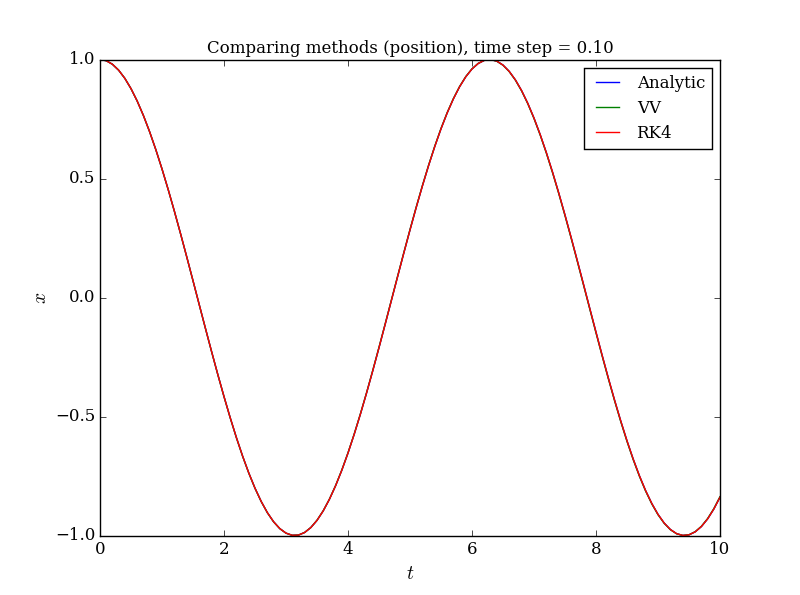
\includegraphics[width=60mm]{Images/comparison_x_01.png}
	& 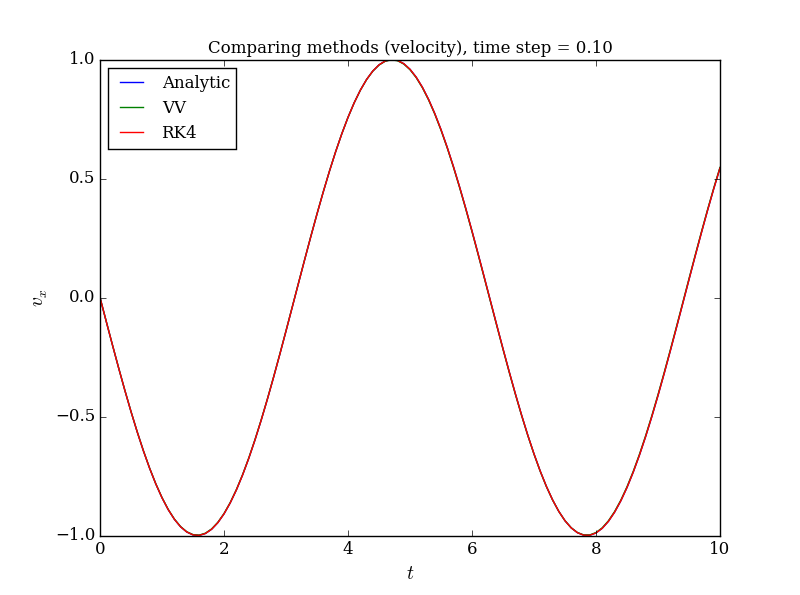
\includegraphics[width=60mm]{Images/comparison_v_01.png}
	& 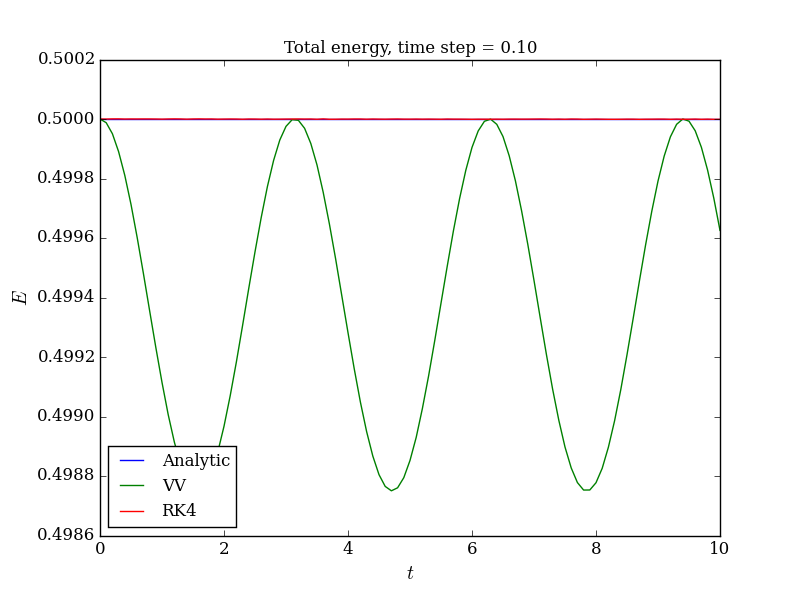
\includegraphics[width=60mm]{Images/comparison_E_01.png} \\
	(a) Position, $\Delta t = 0.10$, $t_{\mathrm{final}} = 10$		& (b) Velocity, $\Delta t = 0.10$, $t_{\mathrm{final}} = 10$  	& (c) Energy, $\Delta t = 0.10$, $t_{\mathrm{final}} = 100$ \\[6pt]
	
	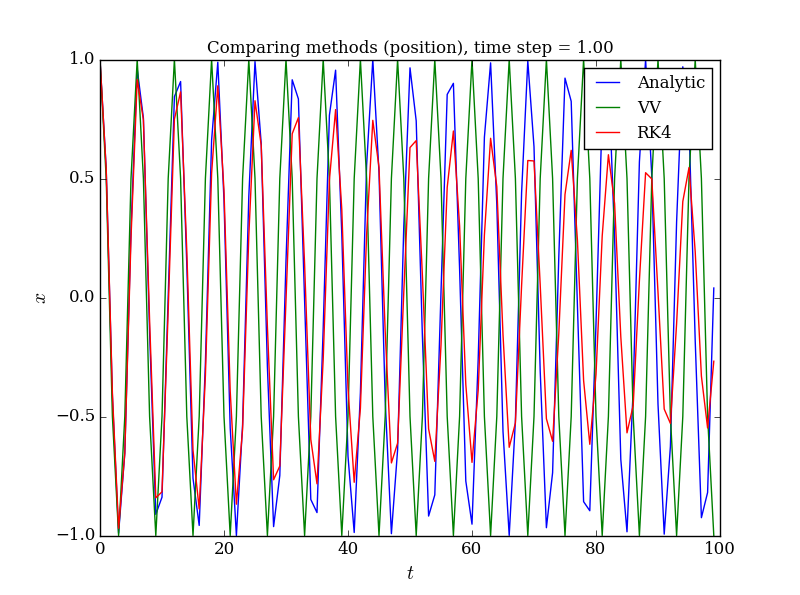
\includegraphics[width=60mm]{Images/comparison_x_1.png} 
	& 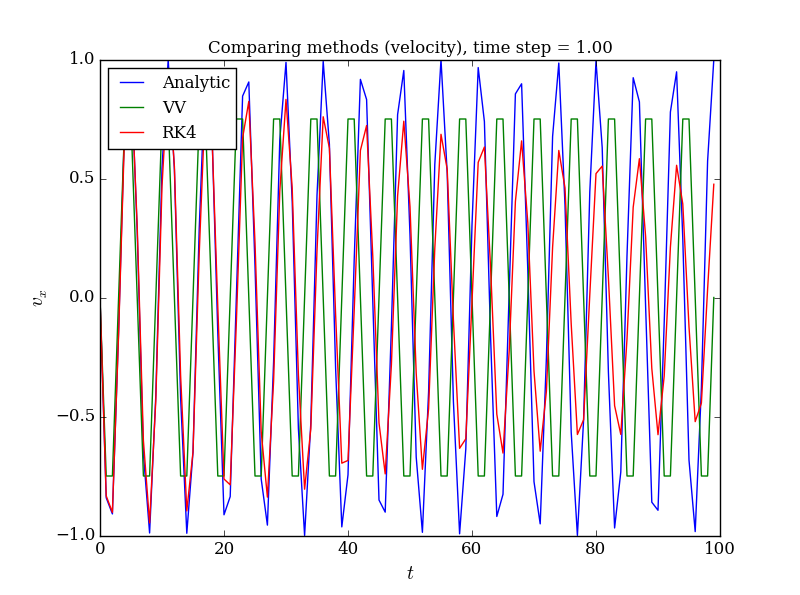
\includegraphics[width=60mm]{Images/comparison_v_1.png}
	& 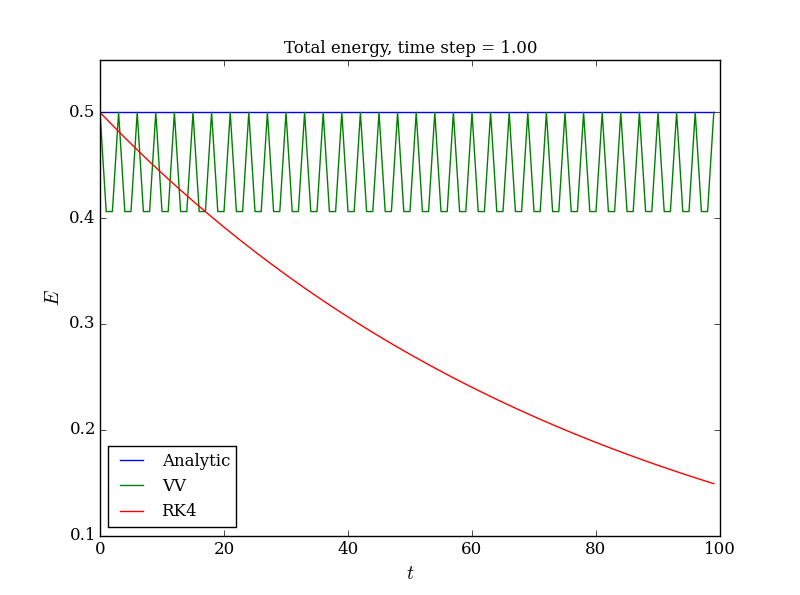
\includegraphics[width=60mm]{Images/comparison_E_1.png} \\
	(d) Position, $\Delta t = 1.00$, $t_{\mathrm{final}} = 10$ 		& (e) Velocity, $\Delta t = 1.00$, $t_{\mathrm{final}} = 10$		& (f) Energy, $\Delta t = 1.00$, $t_{\mathrm{final}} = 100$  \\[6pt]
\end{tabular}
\caption{Comparison of our numerical algorithms in the analytical case of the box on a spring: Velocity-Verlet (green) and 4th-order Runge-Kutta (red), with the analytical solution (blue) are shown for two different time steps $\Delta t = 0.10$ and $\Delta t = 1.00$, and for two different durations $t_{\mathrm{final}} = 10$ and $t_{\mathrm{final}} = 100$.}\label{fig:analytical}
\end{center}
\end{figure*}


\noindent Now that we have verified our numerical methods, we can go on to solve the problem at hand.



\subsection{Stability of methods}

% Spring force
Let us first comment on the stability of the analytical case before moving on to the gravitational system. Studying the analytical case with spring force, the two methods described in Sec.~\ref{sec:methods} are good estimates for time step $\Delta t<1$. RK4 is slightly closer to the analytical solution. For $\Delta t \geqslant 1$, the oscillation in position and velocity is damped when using RK4. This is more visible for longer times. With the VV method, the position amplitude is 1, whereas the velocity amplitude is lowered to 0.75. Thus, for larger time steps, VV is the most stable method.

% 2-body problem
Now let us consider the Newtonian two-body problem in three dimensions. Here we have chosen a configuration similar to that of the Sun-Earth system: One mass is heavy ($M = 1 M_{\odot}$) and has no velocity of its own (Sun), while the other mass is much lighter ($M = 1 M_{\bigoplus} = 0.000003 M_{\odot}$) with some orbital velocity (Earth). In this scenario we can use that $GM_{\odot} = 4\pi^2$ AU$^3$/years$^2$. By letting Earth sit at a distance 1 AU from the Sun and giving the planet a velocity close to that of the Earth which is 29.78 km/s, we get a system where our Earth-like object follows a nice orbit around the massive object in the center. 

As seen in Fig.~\ref{fig:2_body}a-d, the orbit -- or lack thereof -- very much depends on the time step. If the time step is too small, $\Delta t = 0.5$ years in this case, no stable orbit is achieved, though RK4 is hinting at an orbit in Fig.~\ref{fig:2_body}a. For a smaller time step of $\Delta t = 0.05$ years, what originally looks like nice Earth orbits are obtained, though the VV orbit is slowly increasing drifts with time, as seen in Fig.~\ref{fig:2_body}e. However, for a time step of $\Delta t = 0.005$ years, both methods give stable orbits, both for short and long time scales, as seen in Fig.~\ref{fig:2_body}c and Fig.~\ref{fig:2_body}f. $\Delta t = 0.005$ years is thus the best time step to use in this case, and based on Fig.~\ref{fig:2_body}b and Fig.~\ref{fig:2_body}e, RK4 appears to be the more stable of the two methods. $\Delta t = 0.005$ years translates into 1.8 days.

\begin{figure*}
\begin{center}
\begin{tabular}{ccc}
  	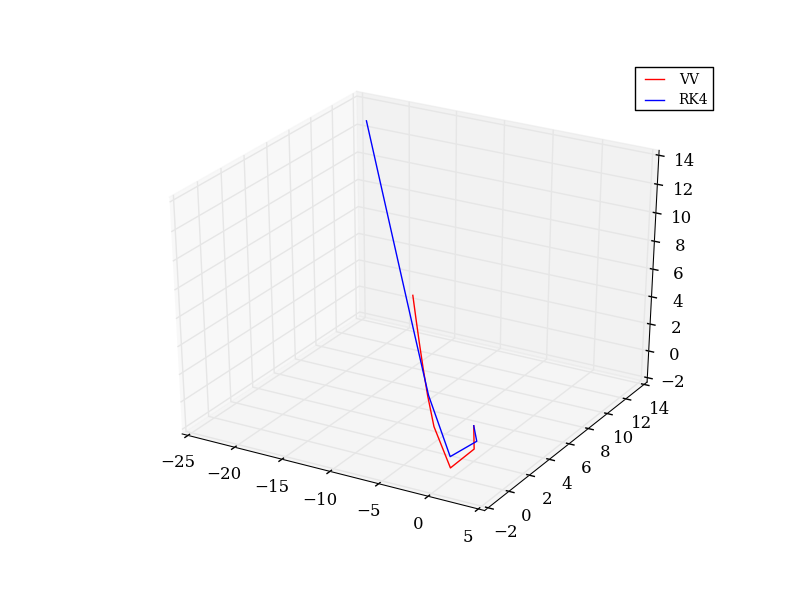
\includegraphics[width=60mm]{Images/Earth-Sun/EarthSun_orbit_05_tfinal5.png}
	& 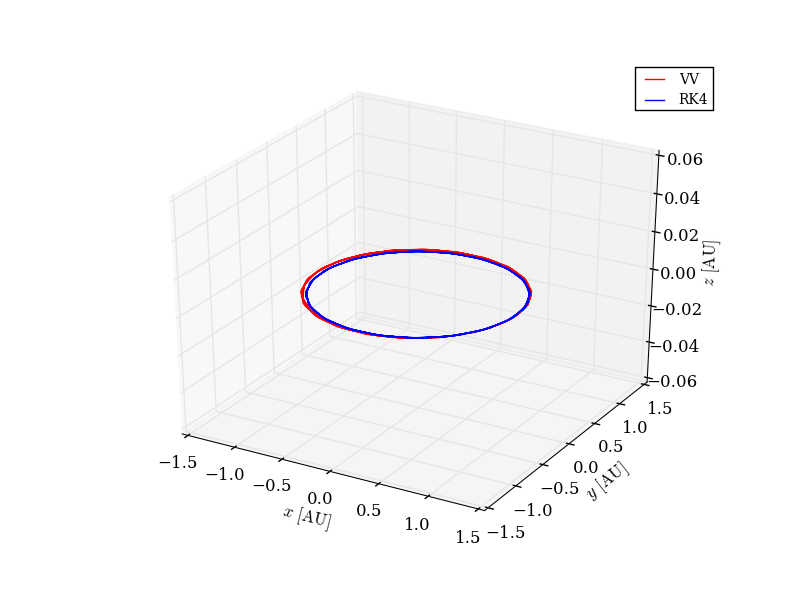
\includegraphics[width=60mm]{Images/Earth-Sun/EarthSun_orbit_005_tfinal5.png} 
	& 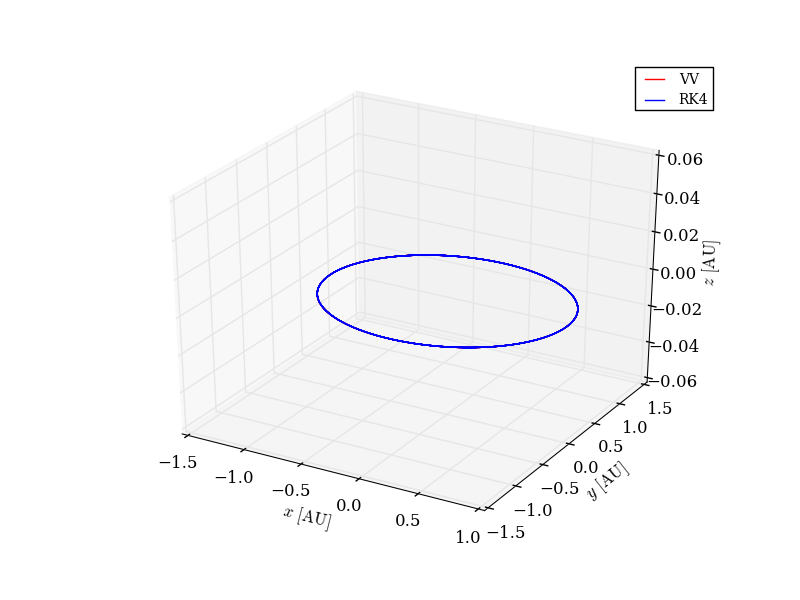
\includegraphics[width=60mm]{Images/Earth-Sun/EarthSun_orbit_0005_tfinal5.png}\\
	(a) $\Delta t = 0.5$ years, $t_{\mathrm{final}} = 5$ years		& (b) $\Delta t = 0.05$ years, $t_{\mathrm{final}} = 5$ years  	& (c) $\Delta t = 0.005$ years, $t_{\mathrm{final}} = 5$ years\\[6pt]
	
	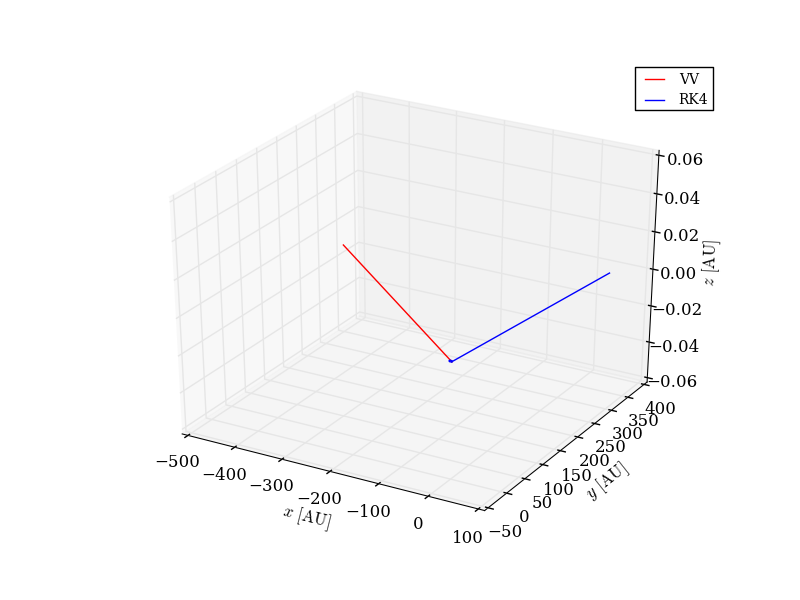
\includegraphics[width=60mm]{Images/Earth-Sun/EarthSun_orbit_05_tfinal50.png}
	& 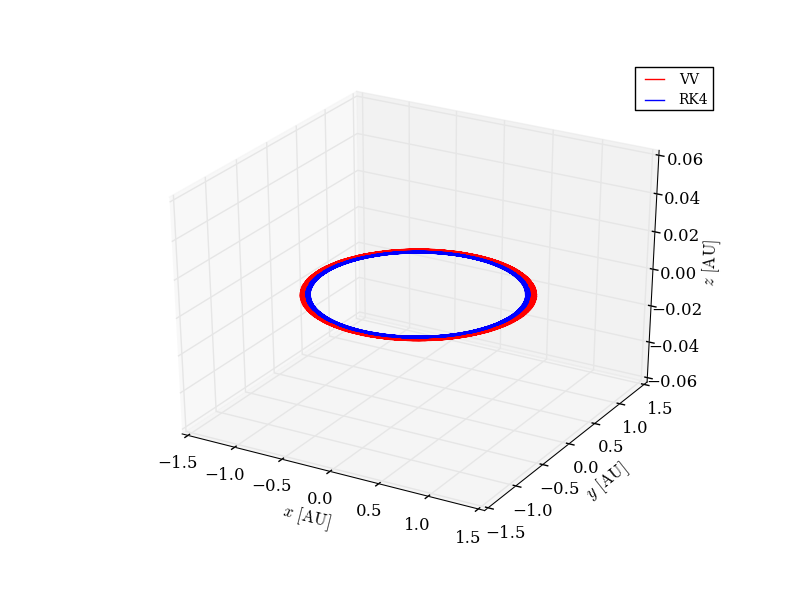
\includegraphics[width=60mm]{Images/Earth-Sun/EarthSun_orbit_005_tfinal50.png}
	& 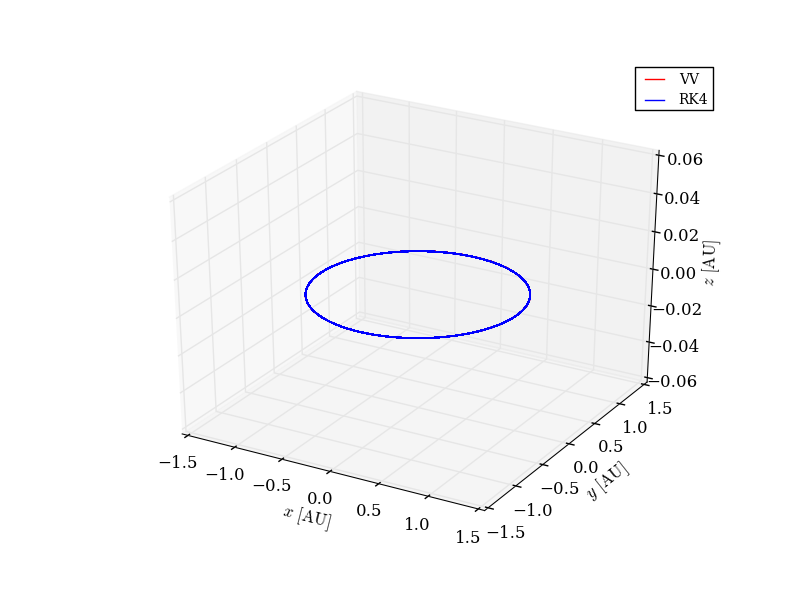
\includegraphics[width=60mm]{Images/Earth-Sun/EarthSun_orbit_0005_tfinal50.png} \\
	
	(d) $\Delta t = 0.5$ years, $t_{\mathrm{final}} = 50$ years		&(e) $\Delta t = 0.05$ years, $t_{\mathrm{final}} = 50$ years 	& (f) $\Delta t = 0.005$ years, $t_{\mathrm{final}} = 50$ years  \\[6pt]
\end{tabular}
\caption{Orbits for our two numerical algorithms in the 2-body case where one body is massive and sitting in the center of the orbit (not plotted): Velocity-Verlet (red) and 4th-order Runge-Kutta (blue) for different time steps $\Delta t$, and two different final times $t_{\mathrm{final}} = 5$ and $t_{\mathrm{final}} = 50$. Axes are in AUs.}\label{fig:2_body}
\end{center}
\end{figure*}
Also of interest is to compare the time used by the two numerical methods to see which one is the most efficient. Instead of quoting the time used to compute \textit{one} time step, we here quote the time taken by the calculation as a whole. See Table~\ref{table:times}. Here we have used $t_{\mathrm{final}} = 1.0$. In the 2-body case (we will get back to the 100-body case later) we see that the time usage is very similar for the two methods, increasing by a factor of 10 when the number of integration points is increased by a factor of 10. The times quoted here does however differ from run to run, where the first digits -- if rewriting to scientific notation -- typically range from 1.5 to 2.6. It also happens that which of the methods is the fastest one changes. In conclusion, the time differences for the two methods are too small for timing to be an issue for choosing one of the methods over the other considering the 2-body case.

\begin{table*}
\begin{center}
\begin{tabular}{ l l l l l l}\hline
	$\Delta t$ 				& Integration points	 	& Time: 2-body RK4			& Time: 2-body VV			& Time: 100-body RK4 		& Time: 100-body VV	\\ \hline
	0.0001 				& $10\,000$ 			& 0.168853				& 0.157352				& 22.0822					& 18.539		 \\
	0.001 				& $1\,000$ 			& 0.020674				& 0.021062				& 2.10406					& 1.78809		 \\
	0.01 					& $100$ 				& 0.002490				& 0.002334				& 0.220827				& 0.171404	 \\
	0.1 					& $10$				& 0.000165				& 0.000147				& 0.02771					& 0.018001		 \\
	\hline
\end{tabular}
\caption{The time (in seconds) spent running the calculations for the two different numerical methods in the 2-body and 100-body cases.}\label{table:times}
\end{center}
\end{table*}

In conclusion, based on our study of the stability and time usage of the two methods, RK4 appears to be the better choice of method when simulating systems that require long times, though it does not matter much which method we choose when the time step is sufficiently small, according to Fig.~\ref{fig:2_body}c and Fig.~\ref{fig:2_body}f, as well as the results in Table~\ref{table:times}.



\subsection{Evolution of the $N$-body system}
We go on to study the $N$-body system where we use a dimensionless $G$ as described in Sec.~\ref{sec:nondim} and treat the system in units of light years and $\tau_{\mathrm{crunch}}$. 

For a system with $N = 100$ objects and a radius $R_0$ = 20 ly, we would first like to know how large the time steps are required to be for the methods to produce good results. First we note that $\tau_{\mathrm{crunch}} = 250$ million years, comparable to the general life time of a non-massive open cluster being only a few hundred million years. We run the calculations for both methods in Sec.~\ref{sec:methods} for different time steps to see how a change in time step will change the results. This is visualized in Fig.~\ref{fig:N_body_timestep}a-b where we show the effect of varying the time step on the position for both methods on one star in the system. Comparing the positions in Fig.~\ref{fig:N_body_timestep}a and Fig.~\ref{fig:N_body_timestep}b we see that RK4 suffers more dramatically from the change to a larger time step in this case, as apposed to the 2-body case, while VV keeps its shape impressively well.

Time spent running the two methods is also something to consider. Let us revisit Table~\ref{table:times}. In the 100-body case it is now more clear, which it was not in the 2-body case, that VV is the fastest of the two methods, however only by a few seconds, making time usage a non-critical issue.

A more critical issue is that of energy conservation. When studying the analytical case it become clear that VV conserves energy, while RK4 does not, as seen in Fig.~\ref{fig:analytical}c and Fig.~\ref{fig:analytical}d.

In conclusion, we see that VV is the better choice of method.  \\


\begin{figure*}
\begin{center}
\begin{tabular}{cc}
  	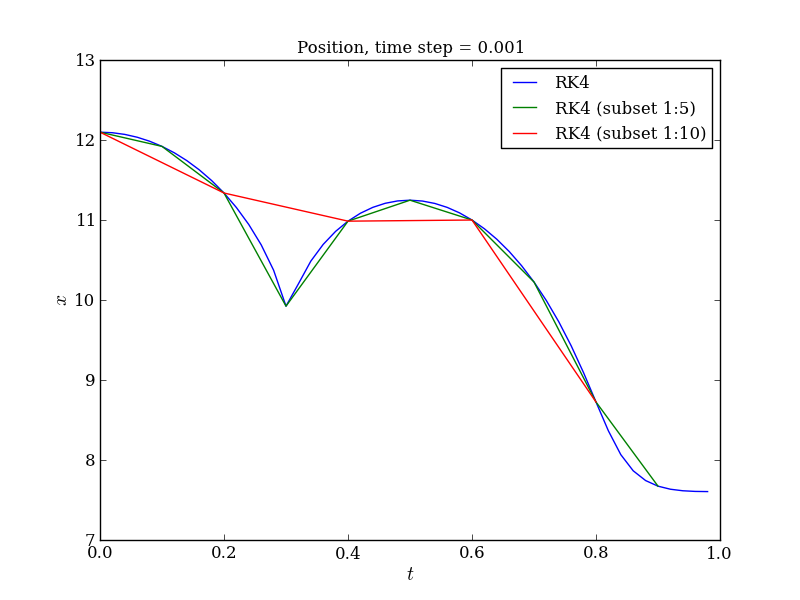
\includegraphics[width=90mm]{Images/comparison_N_RK4_position.png}
	& 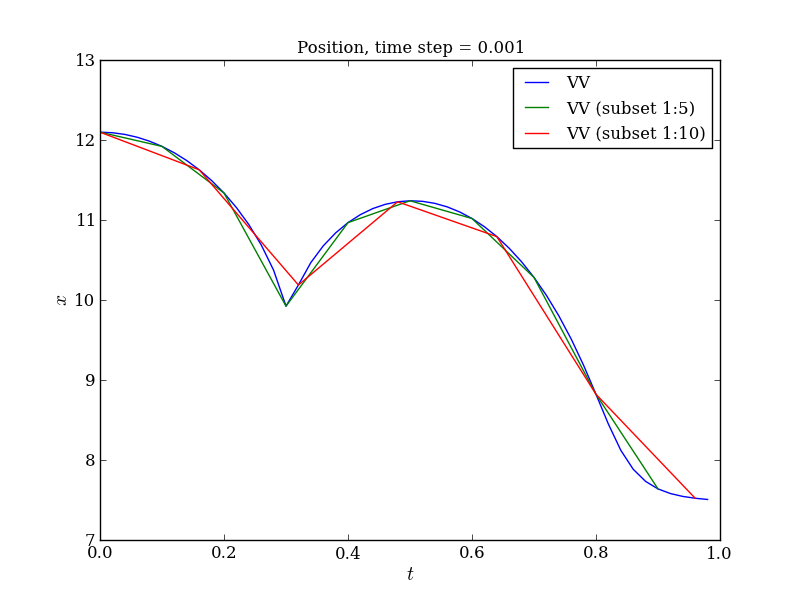
\includegraphics[width=90mm]{Images/comparison_N_VV_position.png} \\
	(a) Position (RK4)				& (b) Position (VV)  \\[6pt]
\end{tabular}
\caption{The decay of precision of RK4 (top) and VV (bottom) for three different time steps $\Delta t \in [0.001, 0.005, 0.025]$ for one of the stars in the $N$-body system.}\label{fig:N_body_timestep}
\end{center}
\end{figure*}

\noindent Now that we have chosen one method, namely the VV method, let us study the system as a whole by plotting the orbits of all the stars. In the case where the number of objects $N \rightarrow \infty$ and the mean density $\rho_0$ of the system is kept constant, the system would collapse into a singularity at a finite \textbf{collapse time}, described in Eq. (\ref{eq:t_crunch}), because it can be considered a continuous fluid. Then each imaginary shell for different radii from the center will be fully filled with stars and feel the same gravitational force towards the center of the system, thus reaching the center at the same time. 

This will not be the case in our model where $N$ is finite. Then the gravitational field will be largely non-uniform, which means the objects will be pulled towards the center of the system and reach it at different times, and keep moving to the other side of the center, instead of all particles gathering in the center at the same time, creating a collapse. This we can see in Fig.~\ref{fig:N_body_simulation}a-i where the system is shown in 3D at initial time, final time and closest to collapse for different values of $N$. It is clear that as $N$ increases, the system will get closer to a real collapse as expected.

The system does not reach an equilibrium where the stars continue in similar orbits over time in the 100-body case, but slowly gets ejected from the system. In the case for higher values like $N = 400$, as seen in Fig.~\ref{fig:N_body_simulation}i, we see that we are approaching an equilibrium solution around $t = 1.84\tau_{\mathrm{crunch}}$ where the stars begins to settle in orbits, however there are still a noticeable number of stars being ejected. 

\begin{figure*}
\begin{center}
\begin{tabular}{ccc}
  	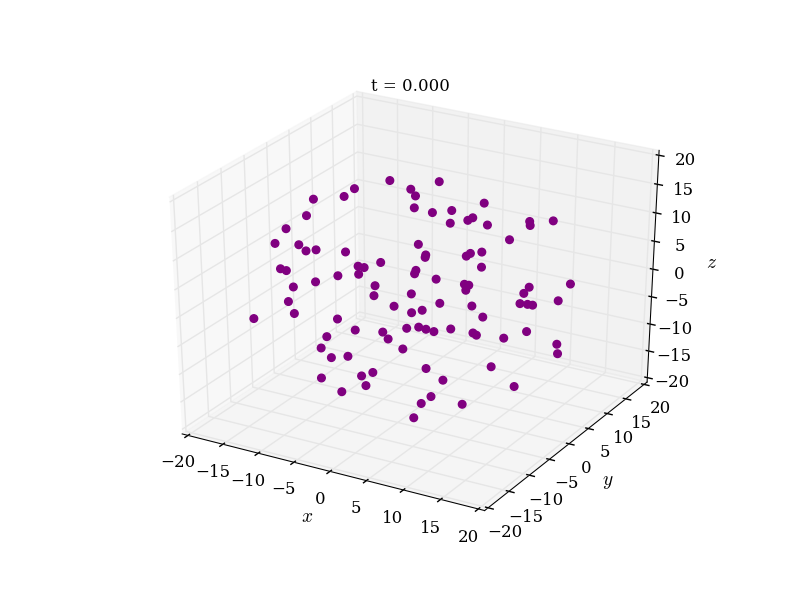
\includegraphics[width=60mm]{Images/Image_100_0000.png}
	& 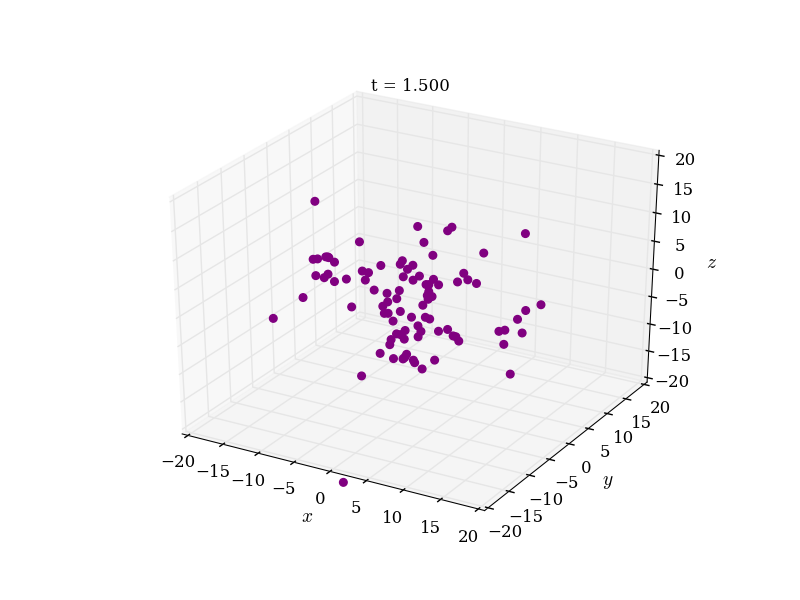
\includegraphics[width=60mm]{Images/Image_100_1500.png}
	& 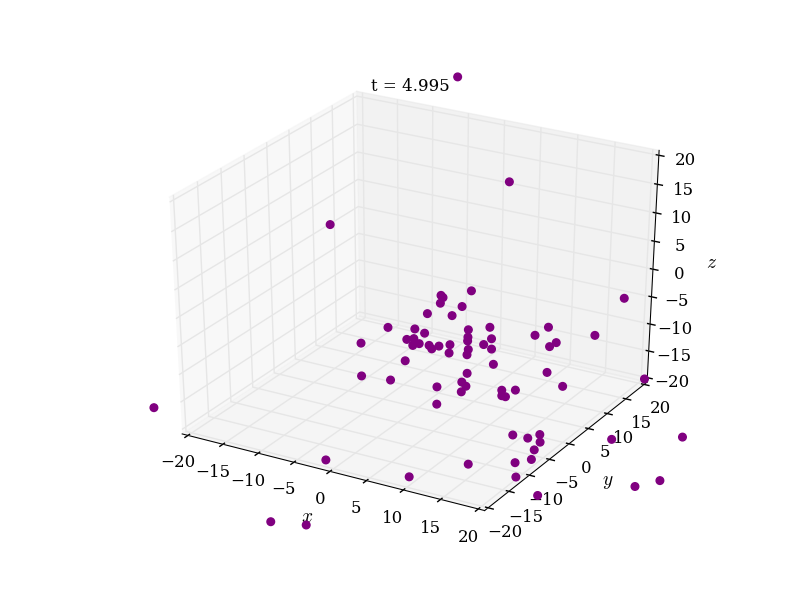
\includegraphics[width=60mm]{Images/Image_100_4995.png} \\
	(a) Initial configuration, $N = 100$				& (b) Closest to collapse at $t = 1.50$, $N = 100$	 	& (c) Final configuration, $N = 100$	 \\[6pt]
	
	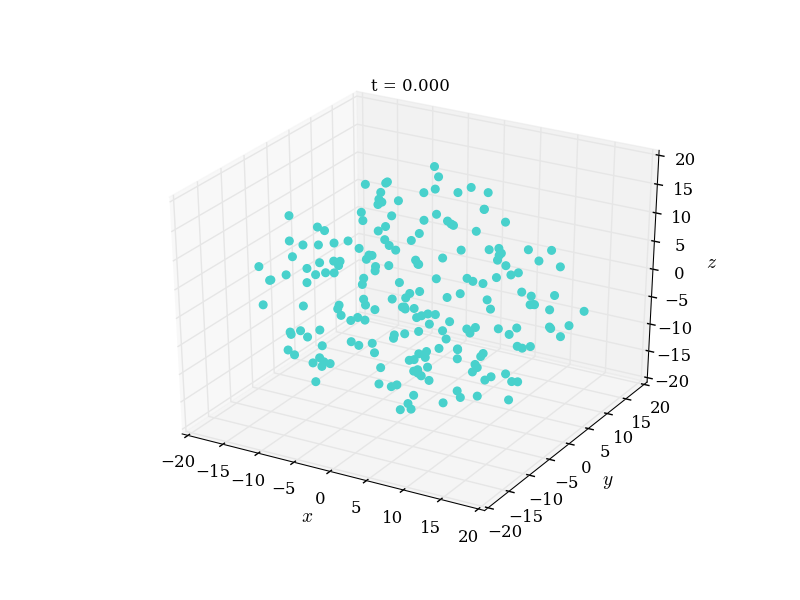
\includegraphics[width=60mm]{Images/Image_200_0000.png}
	& 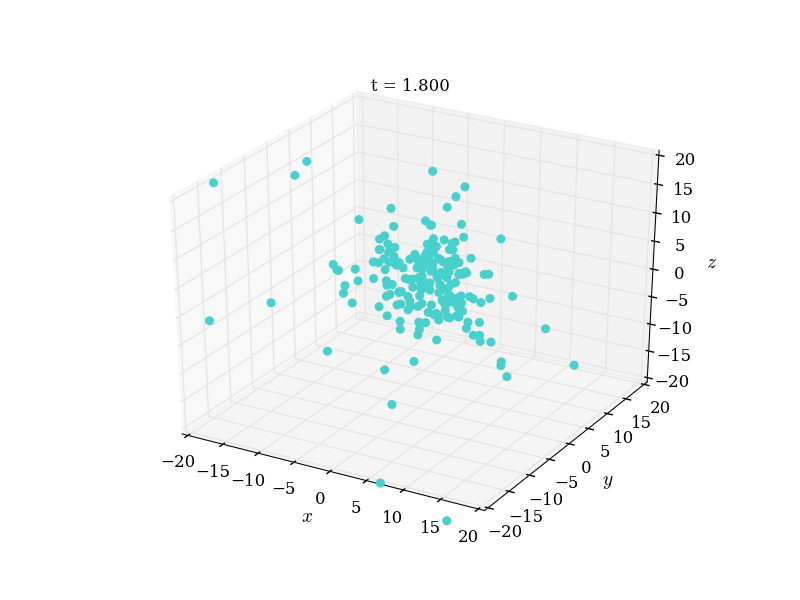
\includegraphics[width=60mm]{Images/Image_200_1800.png}
	& 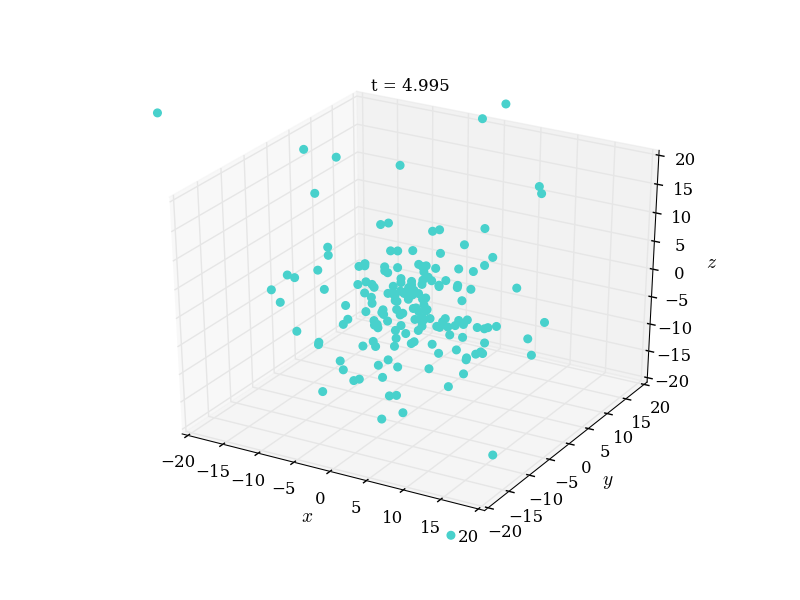
\includegraphics[width=60mm]{Images/Image_200_4995.png} \\
	(d) Initial configuration, $N = 200$					& (e) Closest to collapse at $t = 1.80$, $N = 200$	 	& (f) Final configuration, $N = 200$	 \\[6pt]
	
	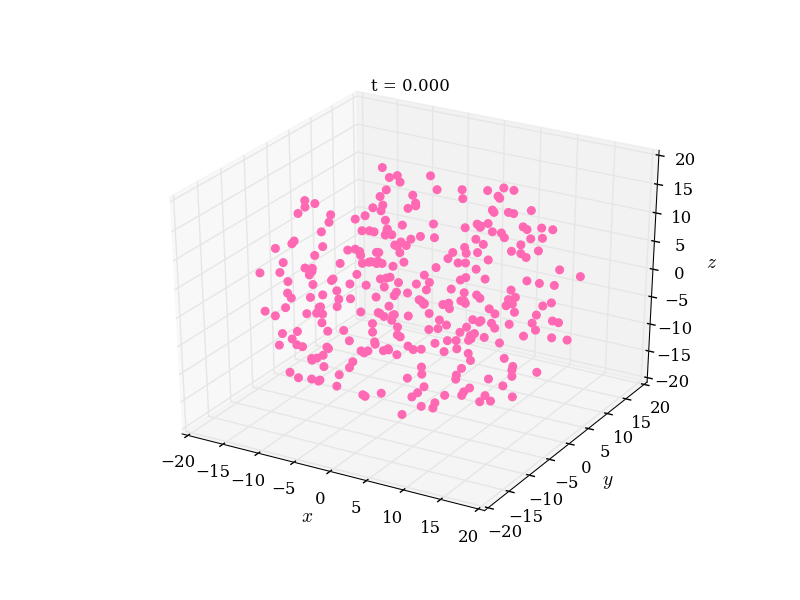
\includegraphics[width=60mm]{Images/Image_300_0000.png}
	& 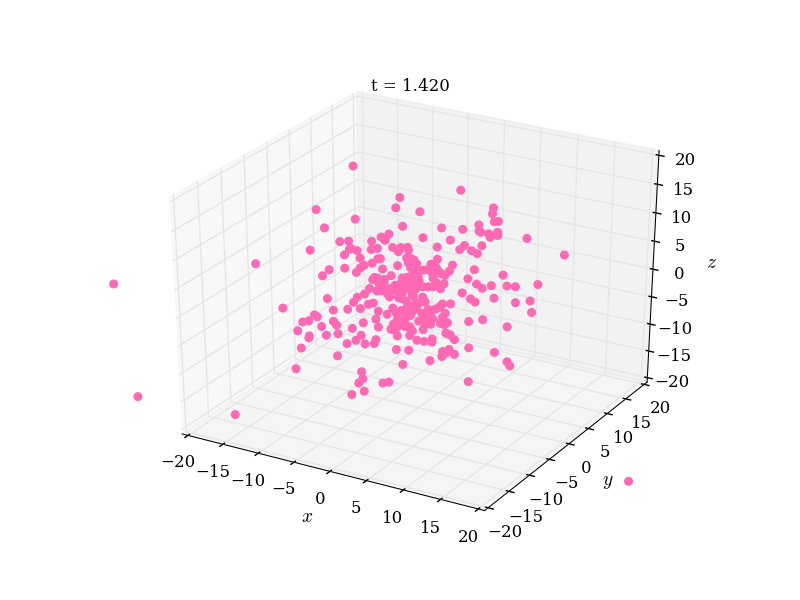
\includegraphics[width=60mm]{Images/Image_300_1420.png}
	& 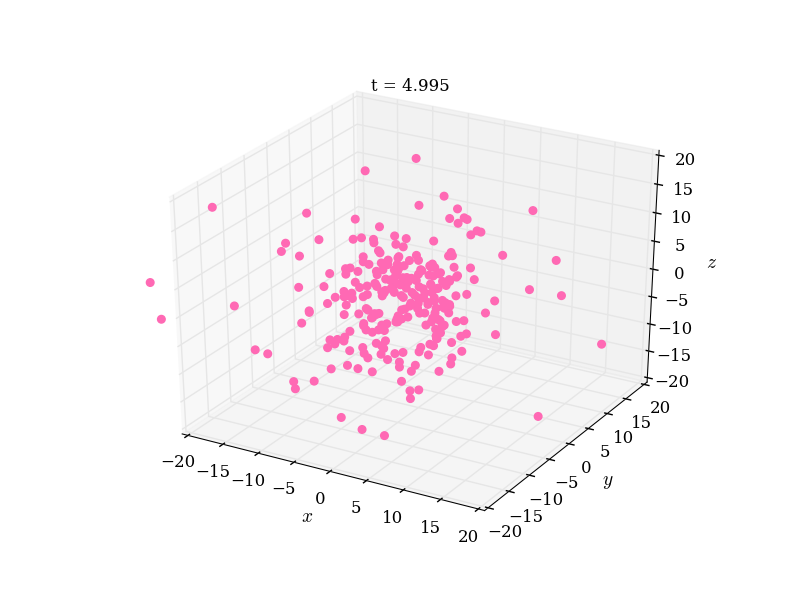
\includegraphics[width=60mm]{Images/Image_300_4995.png} \\
	(g) Initial configuration, $N = 300$					& (h) Closest to collapse at $t = 1.420$, $N = 300$	 	& (i) Final configuration, $N = 300$	 \\[6pt]
	
	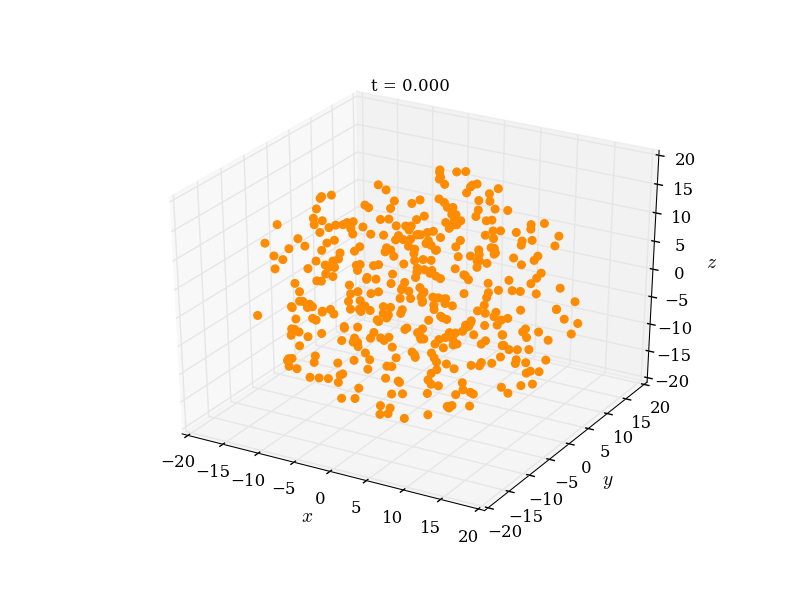
\includegraphics[width=60mm]{Images/Image_400_0000.png}
	& 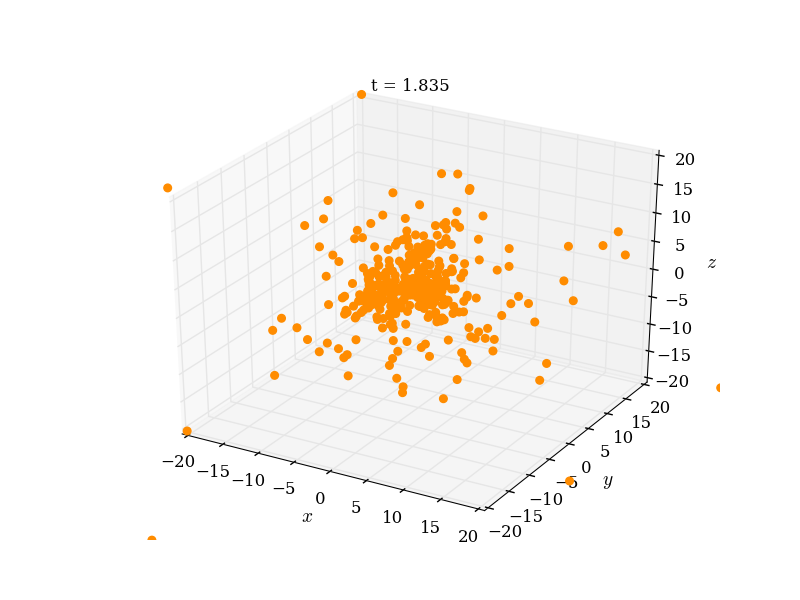
\includegraphics[width=60mm]{Images/Image_400_1835.png}
	& 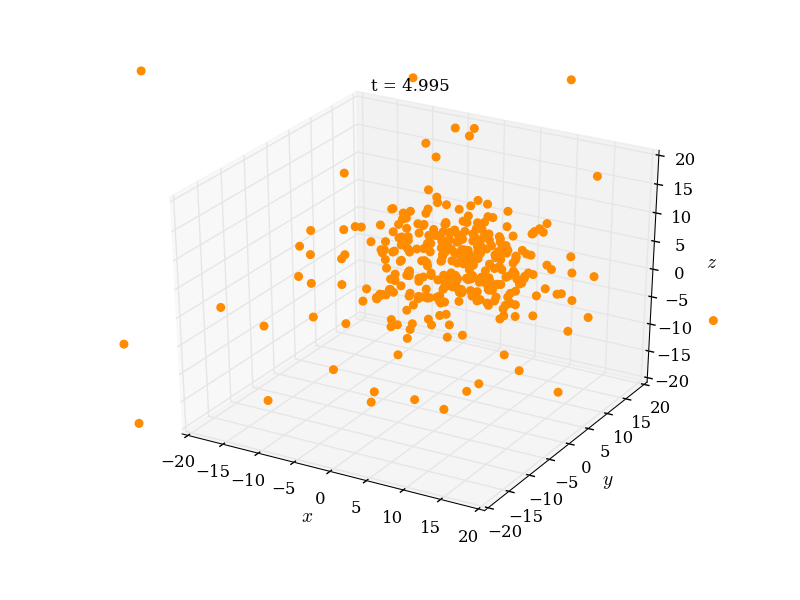
\includegraphics[width=60mm]{Images/Image_400_4995.png} \\
	(g) Initial configuration, $N = 400$					& (h) Closest to collapse at $t = 1.84$, $N = 400$	 	& (i) Final configuration, $N = 400$	 \\[6pt]
\end{tabular}
\caption{Evolution of the $N$-body system as a function of time for a total of 5$\tau_{\mathrm{crunch}}$ for three different values of $N$.}\label{fig:N_body_simulation}
\end{center}
\end{figure*}




\subsubsection{The energy of the system}

We calculate the kinetic and potential energy of our system to study whether the energy is conserved, and see if this is dependent on the number of objects $N$, using

\begin{equation}\label{eq:E_tot}
	E = \frac{1}{2}Mv^2 - \frac{GMm}{r}
\end{equation}
where $M$ is the mass of the star we are considering and $m$ is the mass of another star exerting a gravitational force on our stars. The first term represents the kinetic energy and the second term represents the potential energy due to gravity.

Fig.~\ref{fig:Nbody_energy}a-f shows the kinetic and potential energy for the system of stars, where we have excluded the energy contributions from stars that have been ejected from the system. An ejected star is identified by comparing its kinetic and potential energy. If its kinetic energy is the larger of the two, the star will have a velocity large enough to escape the gravitational field, i.e. a large enough escape velocity.

The kinetic energy rises quickly in the beginning of the simulation, as seen in Fig.~\ref{fig:Nbody_energy}a-c, then stabilizing around $t = \tau_{\mathrm{crunch}}$. The figure closely resembles Fig. 4 in Joyce \textit{et. al} (2010). The overall kinetic energy decreases for larger values of $N$. This corresponds to what we saw in the scatter plots in Fig.~\ref{fig:N_body_simulation}a-i where the collection of stars appear to be more tightly bound for higher values of $N$ at the end of the simulation, corresponding with an increasing potential energy.  

The potential energy in Fig.~\ref{fig:Nbody_energy}d-f is steadily increasing as the stars are pulled towards the center. These plots show a maximum at $t \in [2.2, 2.5, 1.5] \tau_{\mathrm{crunch}}$ for $N = 100,200,300$ respectively, corresponding to the time at which the stars are closest to collapse. The fact that there is a peak in these plots, indicates that they system does not stay nicely bound in the center of the sphere, but that the stars instead crossed the center and keeps moving to the other side, making the system expand again.

In the case of $N = 300$ both the kinetic and potential energy stabilizes at around $t = 1.5\tau_{\mathrm{crunch}}$, approaching an equilibrium situation. 

We also tried running the calculations for $N = 500$, but is resulted in memory error when plotting the results with Python. We have therefore limited ourselves to $N = 300$. 

\begin{figure*}[t!]
\begin{center}
\begin{tabular}{ccc}
  	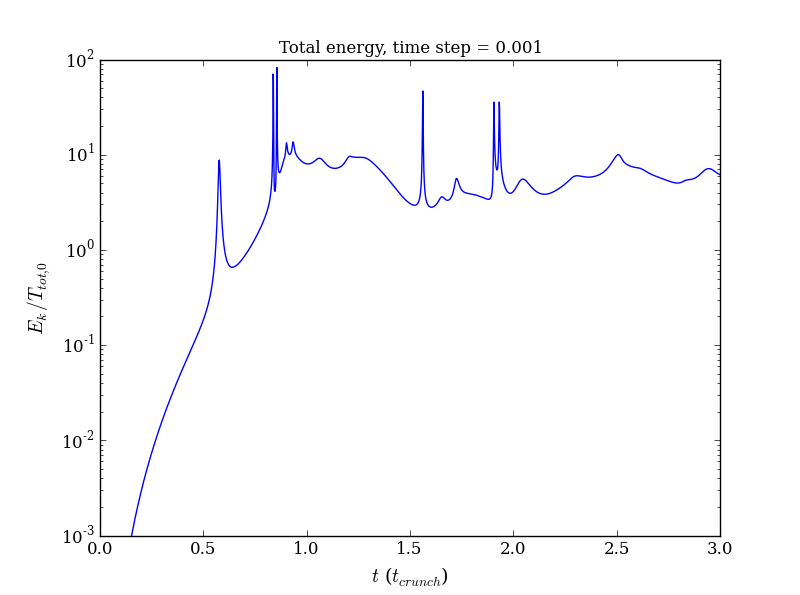
\includegraphics[width=60mm]{Images/Ek_100stars.png}
	& 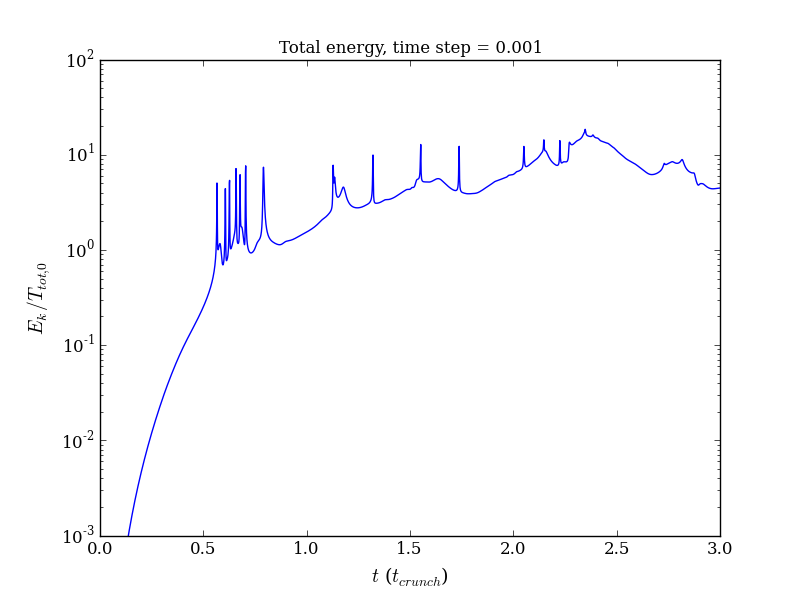
\includegraphics[width=60mm]{Images/Ek_200stars.png}
	& 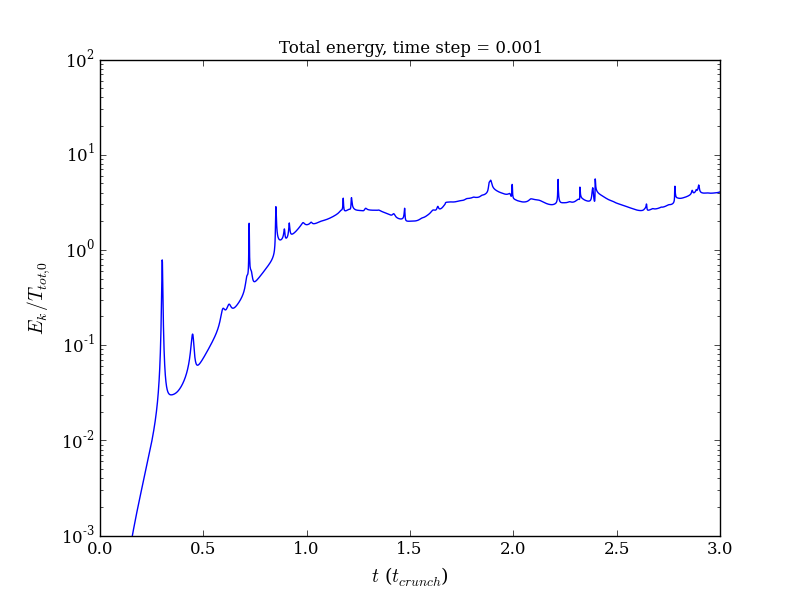
\includegraphics[width=60mm]{Images/Ek_300stars.png} \\
	(a) $N = 100$		& (b) $N = 200$  	& (c) $N = 300$ \\[6pt]
	
	  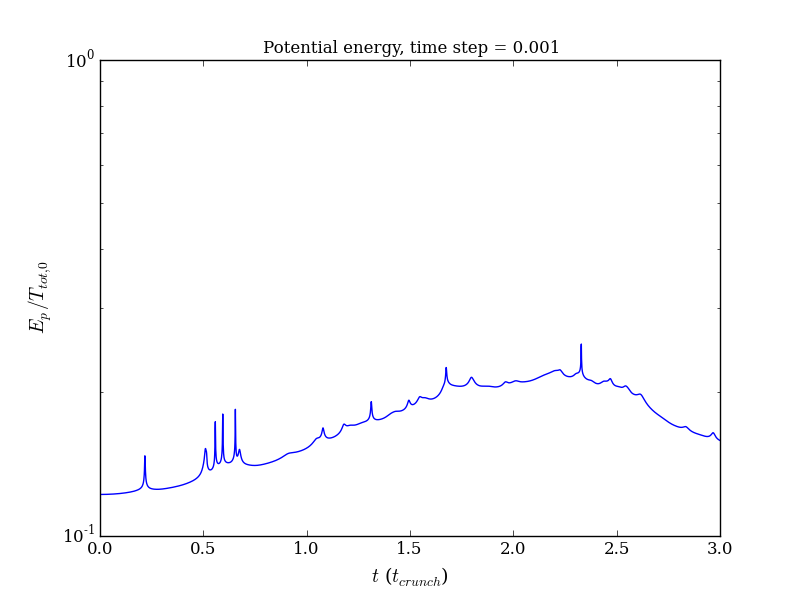
\includegraphics[width=60mm]{Images/Ep_100stars.png}
	& 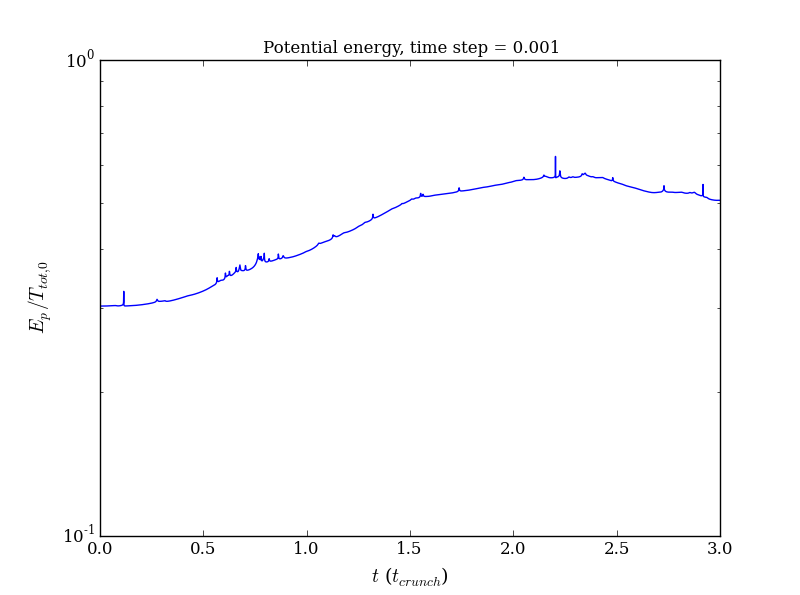
\includegraphics[width=60mm]{Images/Ep_200stars.png}
	& 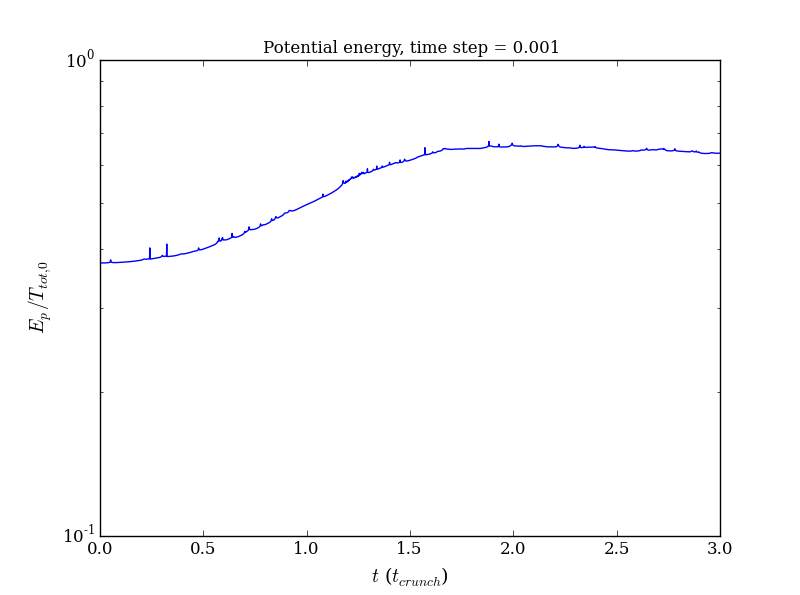
\includegraphics[width=60mm]{Images/Ep_300stars.png} \\
	(d) $N = 100$		& (e) $N = 200$  	& (f) $N = 300$ \\[6pt]
\end{tabular}
\caption{The evolution of kinetic energy (top) and potential energy (bottom) over time for $N = 100, 200, 300$ stars and $\Delta t = 0.001$.}\label{fig:Nbody_energy}
\end{center}
\end{figure*}
How are the energy plots related to the fraction of stars that are ejected from the system? The fraction of ejected stars as a function of time is shown in Fig.~\ref{fig:Nbody_unbound}a for different values of $N$. The shape of the curve closely resembles the curve for the kinetic energy in Fig.~\ref{fig:Nbody_energy}a-c. This is as expected, as the ejected stars are the stars that have large enough velocities to escape, thus contributing the most to the total kinetic energy of the system. 

\begin{figure*}
\begin{center}
\begin{tabular}{cc}
  	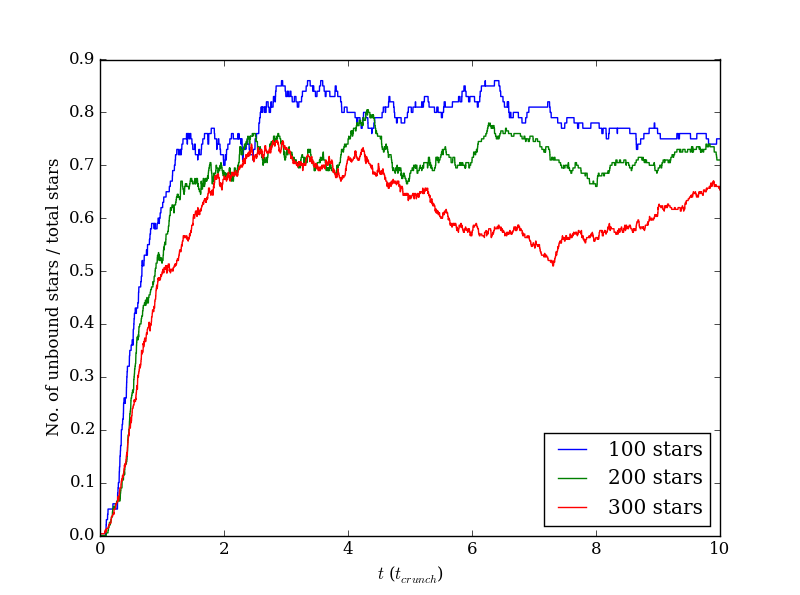
\includegraphics[width=90mm]{Images/unbound_stars.png}
	& 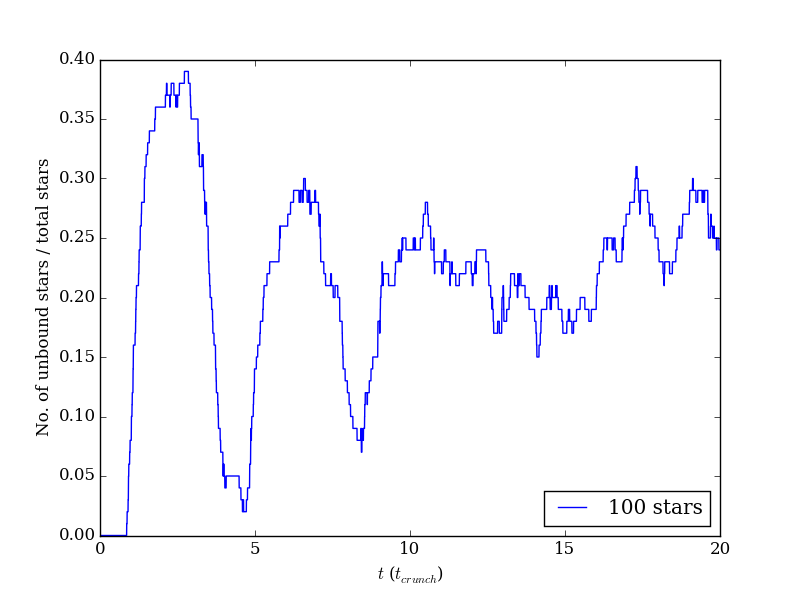
\includegraphics[width=90mm]{Images/unbound_epsilon20.png} \\
	(a) $\epsilon = 0$		& (b) $\epsilon = 20$  \\[6pt]
\end{tabular}
\caption{Fraction of unbound stars as a function of time for different values of $N$ in the un-smoothed (a) and smoothed case (b).}\label{fig:Nbody_unbound}
\end{center}
\end{figure*}
A thing to note is that the fraction of ejected stars oscillates quite a bit. The fraction of ejected stars peaks around $t = 2\tau_{\mathrm{crunch}}$ in all cases. In the case of $N = 300$ the fraction decreases quite significantly after this point and then starts increasing again after $t = 7\tau_{\mathrm{crunch}}$. This is because we at each time step of our calculations give the stars another chance to be a part of the cluster. This means that stars that originally had reached escape velocity and was on their way out of the system, returns to the cluster. This can happen because several stars can be on their way out in the same direction, pulling on each other, and possibly causing some stars to return to the system. For large values of $N$ this is a more likely scenario, as there are more stars available to produce this effect.




\subsubsection{Introducing the smoothing function and testing the virial theorem}

After running calculations for the gravitational force as expressed in Eq. (\ref{eq:force_comp}), we introduce a \textbf{smoothing function} to take care of any numerical instability that may arise when two stars come very close. Because the gravitational force $F \sim 1/r^2$, we see that the force will become very large as $r \rightarrow 0$, ultimately throwing objects out of the system. 

We modify the gravitational force as

\begin{equation}\label{eq:force_mod}
	F_{G,\mathrm{mod}} = - \frac{G M_1 M_2}{r^2 + \epsilon^2},
\end{equation}
where $\epsilon$ is a small real constant. We will try out different values for $\epsilon$ to see which value gives the best energy conservation.

Adding the value of $\epsilon$ can be understood by noting that we are in reality considering extended objects, rather than point sources. These objects will have a radius $R$, thus the centers of two objects can only get as close as $2R$ to each other. (An alternative approach could be to let objects merge when getting too close.) 

For a bound gravitational system in equilibrium the \textbf{virial theorem} should be fulfilled, which states that

\begin{equation}\label{eq:vir}
	2 \langle K \rangle = - \langle V \rangle,
\end{equation}
where $\langle K \rangle$ is the time-averaged kinetic energy of the system and $\langle V \rangle$ is the time-averaged potential energy of the system. By calculating the kinetic and potential energy of the stars in our system that are bound (not ejected), we can check if our results are consistent with the virial theorem and use this as an indication of which value of $\epsilon$ is better.

By trying out different values of $\epsilon$, we find that the fraction of bound stars fluctuate significantly over time. Whether the virial theorem is fulfilled or not also fluctuate. From many trials, $\epsilon = 20$ stands out as a good choice. At first suspicious of this value's resemblance to the radius of the sphere $R$ in which our star cluster lives, we checked that this was not the case by testing out $R = \epsilon = 30$. 

It is curious that the value of $\epsilon$ needs to be as large as 20, which will be in units of light years. MORE!!!

In Fig.~\ref{fig:Nbody_unbound}b we see how setting the value of $\epsilon$ to be non-zero affects the evolution of the fraction of unbound stars as a function of time, shown for the 100-body case. Stars are initially thrown out of the system at $t = \tau_{\mathrm{crunch}}$ in large numbers. A very large fraction of these do however return to the system, only to disappear again. The fraction of unbound stars keeps fluctuating, though the amplitude of the fluctuations decrease over time.

If we were only to plot the fraction of unbound stars for times in the range $[0,2.5\tau_{\mathrm{crunch}}]$, Fig.~\ref{fig:Nbody_unbound}b would very much resemble the behavior shown in Fig. 2 in Joyce \textit{et. al} (2010). If we did not allow stars to return to the system, we expect our results to be similar to this figure, which shows a large increase in the fraction of unbound stars at $t = \tau_{\mathrm{crunch}}$, which quickly stabilizes without showing clear fluctuations as our plots do. Here we should also note that Joyce \textit{et. al} (2010) used a system of $N = 10^7$ stars, which is significantly higher than we are capable of.



\subsubsection{Radial profile}

Finally we wish to study the \textbf{radial density} of the particles in the equilibrium state. This can be calculated from our computations and be fitted with the simple expression

\begin{equation}\label{eq:simple_fit}
	n(r) = \frac{n_0}{1 + (\frac{r}{r_0})^4}
\end{equation}
where $n_0$ and $r_0$ are scaling constants. We follow Joyce \textit{et. al} (2010) and approximate these scaling constants with $r_0 \propto N^{-1/3}$ and $n_0 \propto N^2$. The result is shown in Fig. XXXX. 

COMMENTS!

\begin{figure*}
\begin{center}
\begin{tabular}{cc}
  	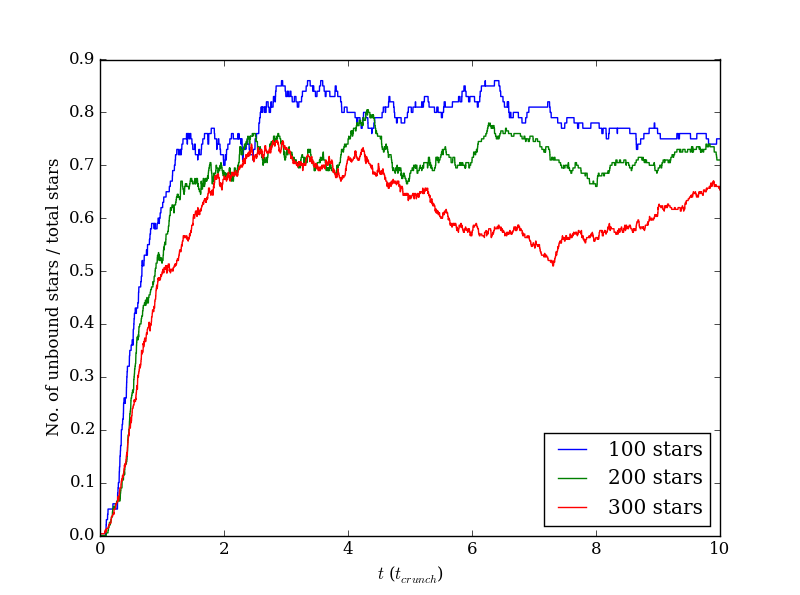
\includegraphics[width=90mm]{Images/unbound_stars.png}
	& 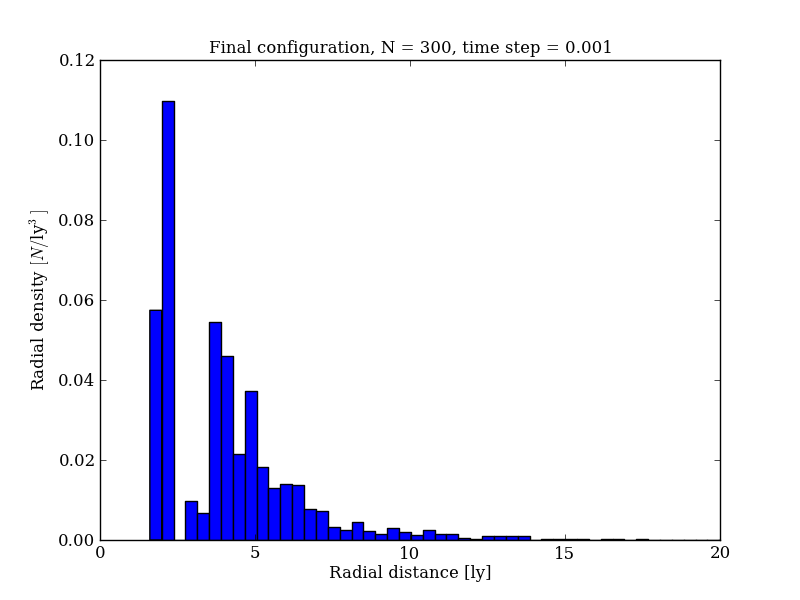
\includegraphics[width=90mm]{Images/histogram_300_epsilon20.png} \\
	(a) $\epsilon = 0$		& (b) $\epsilon = 20$  \\[6pt]
\end{tabular}
\caption{Histogram for radial density as a function of radius for a 300-body system in the un-smoothed (a) and smoothed case (b).}\label{fig:Nbody_histogram}
\end{center}
\end{figure*}


%The result can also be compared with the well-known Navarro-Frenk-White profile
%
%\begin{equation}\label{eq:NFW}
%	\rho(r) = \frac{\rho_0}{  \frac{r}{r_0} (1 + \frac{r}{r_0})^2  },
%\end{equation}
%where $\rho_0$ and $r_0$ are scaling constants, to see if this profile gives a better fit to our data set. 
%
%MORE!!!






\section{Conclusions}\label{sec:conclusion}

We have run an $N$-body simulation of an open star cluster using the 4th order Runge-Kutta and Velocity Verlet integration methods. The cluster member began their lives with randomly distributed positions within a sphere with a radius of 20 light years consisting of 100 stars with masses randomly distributed by a Gaussian distribution around ten solar masses with a standard deviation of one solar mass.

Already in the analytical case did we see the bad side of Runge-Kutta methods, which is that these methods do not conserve energy. When simulating a gravitational system, conservation of energy is highly important. This fact, in addition to Velocity Verlet's (VV) accuracy even for larger time steps, led us to make VV our method of choice for our simulations. Time usage by the two methods turn out not to be an issue.

...

An interesting idea for future work would be to include the possibility of stars merging together when sufficiently close to each other.

\section{References}

\begin{enumerate}
	\item Verlet integration methods. (2015, December 9). \\ \verb@https://en.wikipedia.org/wiki/Verlet_integration@
	\item Open cluster. (2015, December 9). \\ \verb@https://en.wikipedia.org/wiki/Open_cluster@
	\item H. T. Ihle. (2015). \textit{On the, not entirely trivial, issue of getting uniformly distributed random coordinates within a sphere.} 
	\item M. Joyce, B. Marcos, and F. Sylos Labini. (2010). \textit{Cold uniform spherical collapse revisited.} AIP Conf. Proc. 1241, 955.
\end{enumerate}



\section{List of codes}

The codes developed and used in this project are: 


\subsection{Running calculations (C++)}

\begin{itemize}
	\item \verb@main.cpp@ -- main program where the calculations are run, calling on the classes listed below. 
	\item \verb@star.cpp@ -- class collecting various properties of the stars.
	\item \verb@galaxy.cpp@ -- class containing all the stars in the galaxy as well as the numerical methods described in Sec.~\ref{sec:methods}.
\end{itemize}


\subsection{Plotting (Python)}

\begin{itemize}
	\item \verb@plotting_analytical.py@ -- program to graphically compare the one-dimensional 2-body problem with an analytical solution, described in Sec.~\ref{sec:analytical_test}.
	\item \verb@plot_methods.py@ -- program to graphically compare the two numerical methods described in Sec.~\ref{sec:RK4} and Sec.~\ref{sec:VV} for the 2-body problem.
	\item \verb@plot_methods_Nbody.py@ -- program to graphically compare the two numerical methods for the $N$-body problem.
	\item \verb@plotting_scatter.py@ -- plotting program to visualize the 3D distribution of particles in the $N$-body system as a scatter plot, as shown in Fig.~\ref{fig:N_body_simulation}. 
	\item \verb@plotting_radialprofile.py@ -- plotting program that calculates the radial profile of the system, fitted with the profile in Eq. (\ref{eq:simple_fit}). %and Eq. (\ref{eq:NFW}).
	\item \verb@t_crunch.py@ -- Short program to calculate the value of $\tau_{\mathrm{crunch}}$ in units of years for the $N$-body system.
\end{itemize}




\end{multicols}

\end{document}
